\documentclass[11pt]{article}
\usepackage{geometry}                % See geometry.pdf to learn the layout options. There are lots.
\geometry{a4paper}                   % ... or a4paper or a5paper or ... 
%\geometry{landscape}                % Activate for for rotated page geometry
%\usepackage[parfill]{parskip}    % Activate to begin paragraphs with an empty line rather than an indent
\usepackage{graphicx}
\usepackage{amsmath}
\usepackage{amssymb}
\usepackage{siunitx}
\usepackage{epstopdf}
\usepackage{verbatim}
\usepackage{url}

\DeclareGraphicsRule{.tif}{png}{.png}{`convert #1 `dirname #1`/`basename #1 .tif`.png}


\title{Assignment 3: Hidden Markov Models}
\author{\textbf{Sébastien Bouquet}}
\date{}                                           

\begin{document}
\maketitle
\section{Task 1}
\subsection{Point a}
\begin{figure}[!ht]
\center
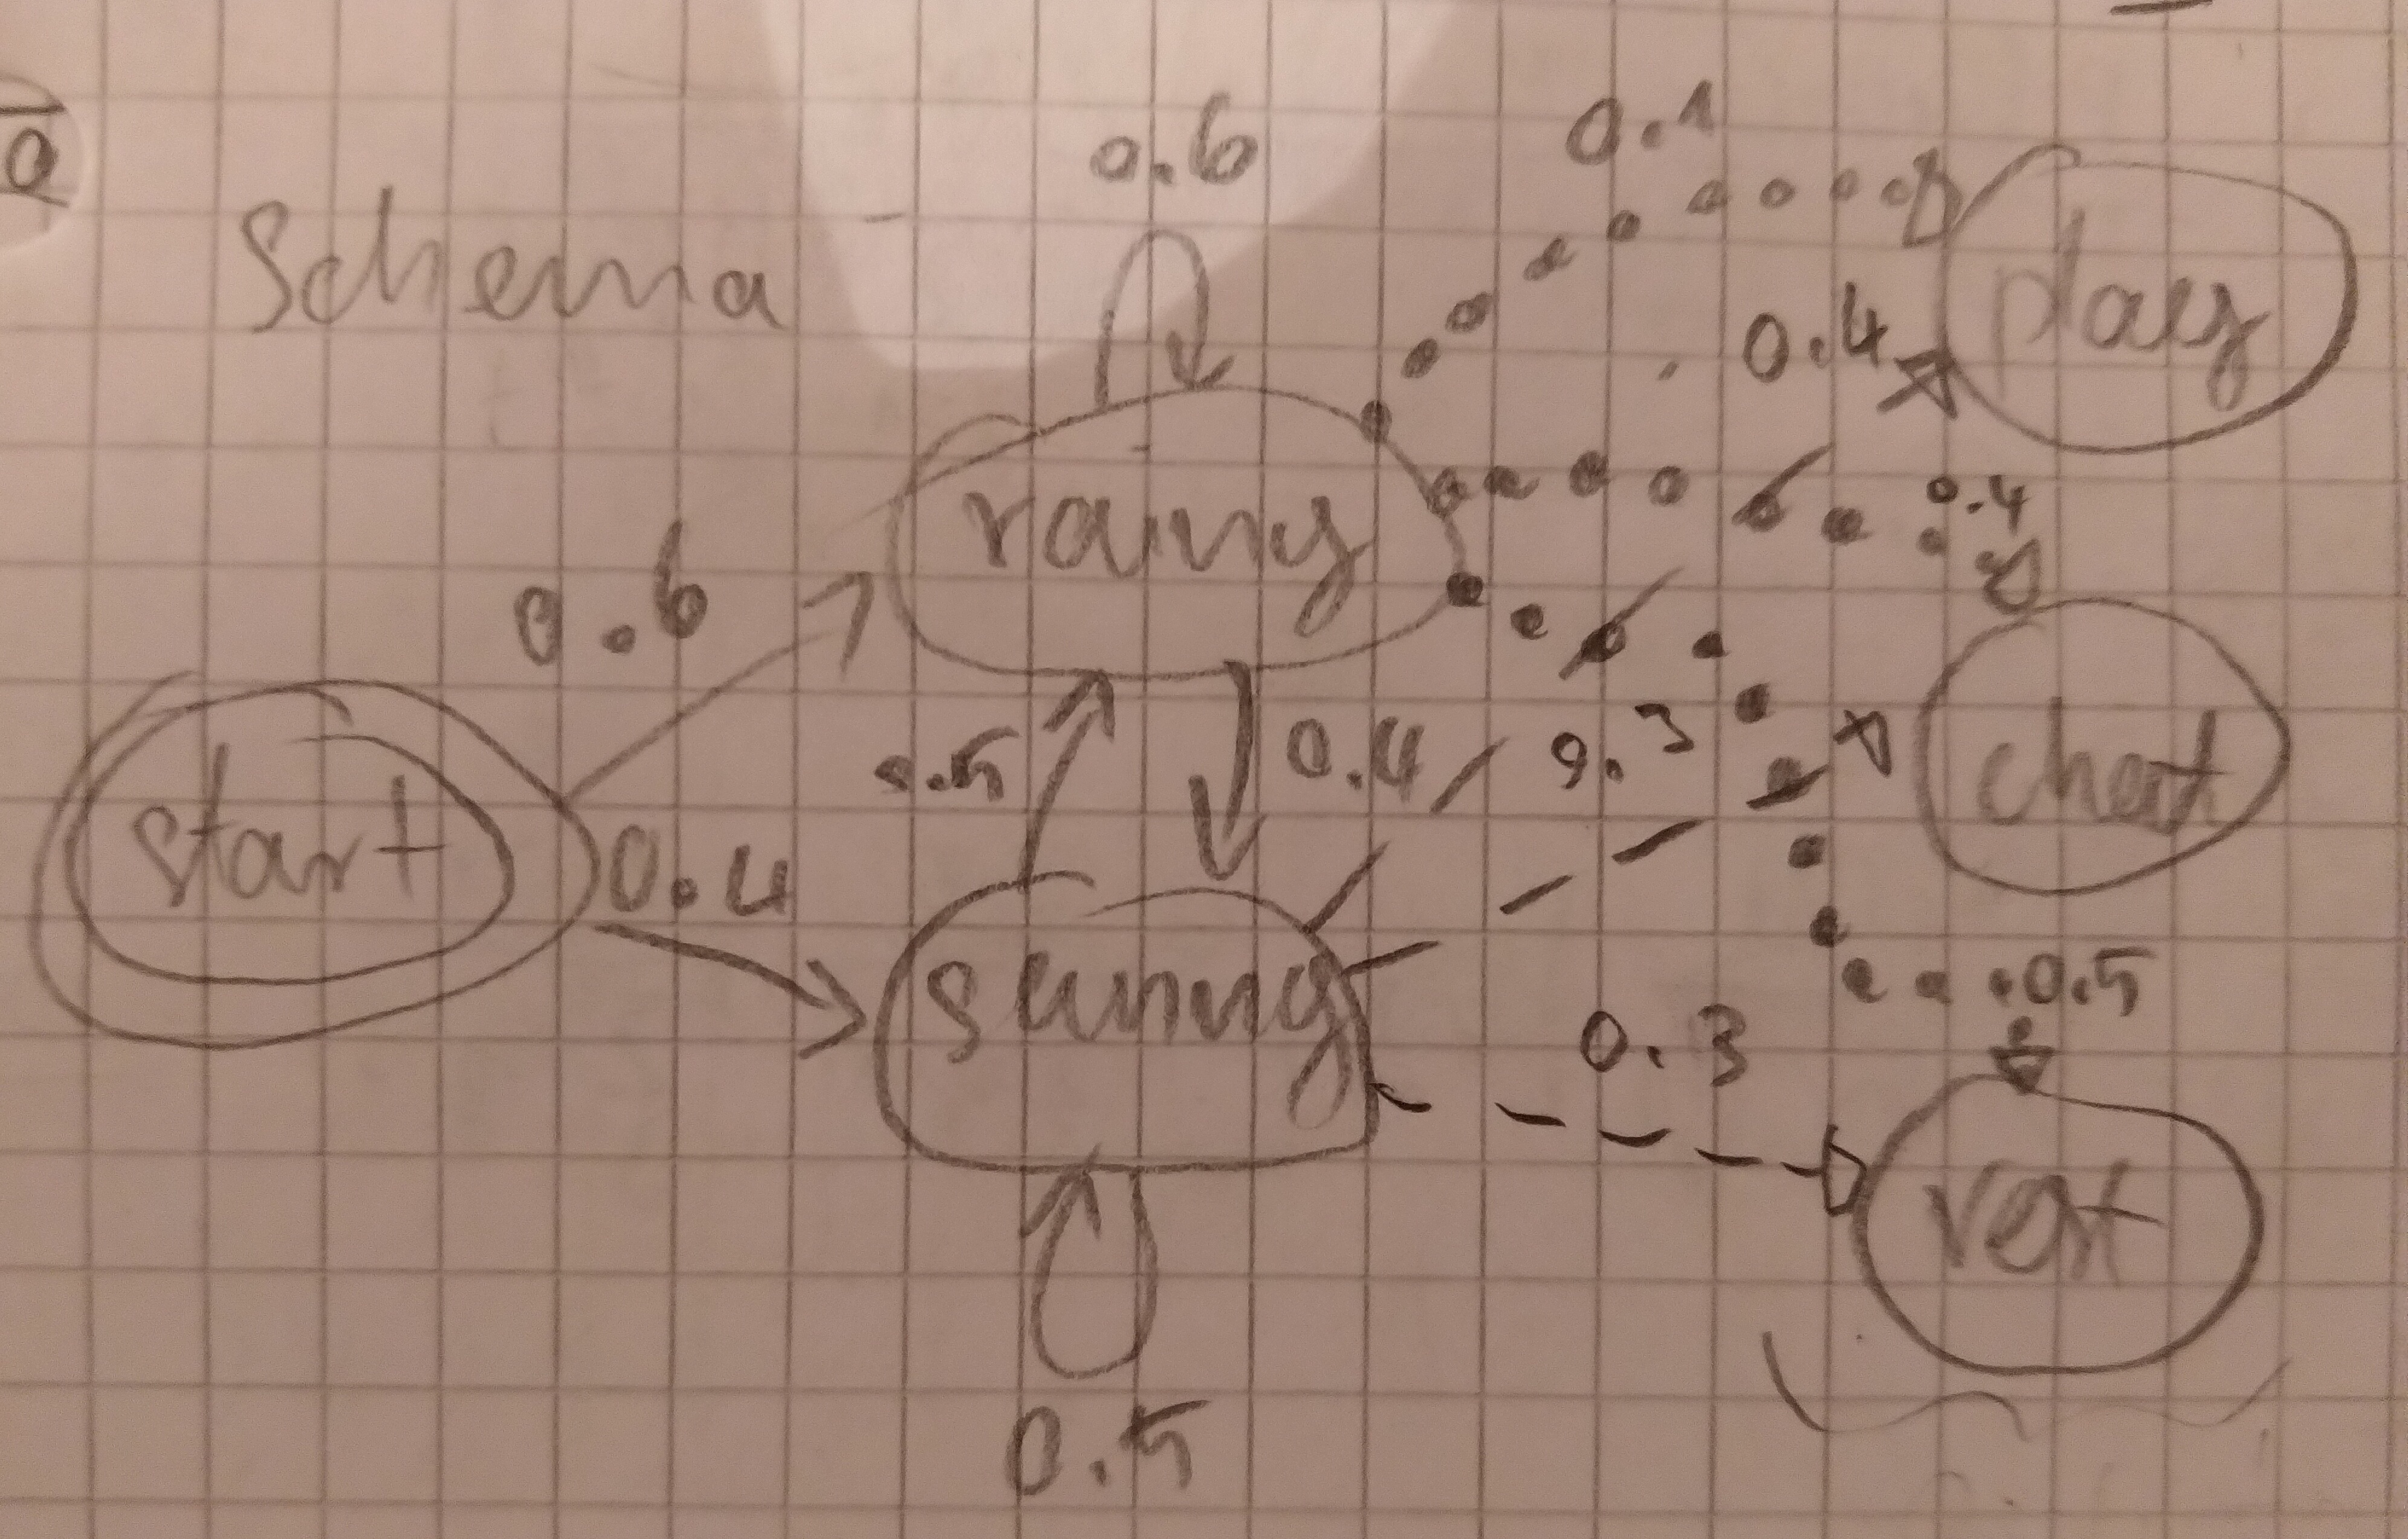
\includegraphics[width=.5\columnwidth]{hmm_task1}
\caption{The HMM model that Sarah may use to estimates the weather in Lugano.}
\label{fig:hmm-task1}
\end{figure}

\subsection{Point b}
The ``stupid way'' of calculating is to use the fact that $P(O_1...O_T| \lambda) = \sum_Q P(O,Q| \lambda) = \sum_Q P(O|Q, \lambda)*P(Q | \lambda)$. Since $P(O|Q, \lambda) = \Pi_{t=1}^T P(O_t | g_t, \lambda)$ and $P(Q | \lambda) = \Pi_{g_1}*a_{g_1g_2}*a{g_2g_3}$, then $P(O_1..O_T|\lambda) = \sum_{g_1,...,g_T} \Pi_{g_1}*b_{g_1}*a_{g_1g_2} * b_{g_2} * ...$. \\ 
In this exercise, we get $P(O_1O_2O_3|\lambda) = \sum_{g_1,g_2,g_3} \Pi_{g_1}*b_{g_1}*a_{g_1g_2}*b_{g_2}*a_{g_2g_3}*b_{g_3}$. \\

($N = \{S, R\} = \{Sunny, Rainy\}$, $O_1=$ chat, $O_2=$ play, $O_3=$ rest) \\
The ``smarter way'' is to use the \textit{forward algorithm}. It is smarter in the sense that the precedent formula has a complexity of $O(T*N^T)$ whereas the \textit{forward algorithm} has a complexity of $O(T*N^2)$. \\
For the \textit{forward algorithm}, we define $\alpha_t(i) = P(O_1O_2O_3, g_t=S_i | \lambda)$. \\
\textbf{Initialization:} \\
$\alpha_1(S) = \Pi_S*b_S(chat) = 0.4*0.3 = 0.12$ \\
$\alpha_1(R) = \Pi_R*b_R(chat) = 0.6*0.4 = 0.24$ \\
\textbf{Update:} \\
$\alpha_2(S) = a_{SS}b_S(play)*\alpha_1(S) + a_{RS}b_S(play)*\alpha_1(R) = 0.5*0.4*0.12+0.4*0.4*0.24 = 0.0624$ \\
$\alpha_2(R) = a_{SR}b_R(play)*\alpha_1(S) + a_{RR}b_R(play)*\alpha_1(R) = 0.5*0.1*0.12 + 0.6*0.1*0.24 = 0.0204$ \\
$\alpha_3(S) = a_{SS}b_S(rest)*\alpha_2(S) + a_{RS}b_S(rest)*\alpha_2(R) = 0.5*0.3*0.0624 + 0.4*0.3*0.0204 = 0.011808 $ \\
$\alpha_3(R) = a_{SR}b_R(rest)*\alpha_2(S) + a_{RR}b_R(rest)*\alpha_2(R) = 0.5*0.5*0.0624 + 0.6*0.5*0.0204 = 0.02172$ \\
\textbf{Termination:} \\
$P(O_1=chat,O_2=plat, O_3=rest | \lambda) = \sum_{i=1}^N \alpha_3(i) = \alpha_3(S) + \alpha_3(R) = \mathbf{0.033528}$

\subsection{Point c}
Using the forward algorithm, we can calculate the most probable final state $g_3$ given the sequence of observations $O_1O_2O_3$: $P(g_3 = S | O_1O_2O_3) = \frac{\alpha_3(S)}{\sum_{i=1}^N \alpha_3(I)} = \frac{0.011808}{0.033528} \approx 0.3522$ \\
$P(g_3 = R | O_1O_2O_3) = \frac{\alpha_3(R)}{\sum_{i=1}^N \alpha_3(I)} = \frac{0.02172}{0.033528} \approx 0.6478 = 1-P(g_3 = S | O_1O_2O_3)$ \\
Thus we find that Sunday was most probably \textit{rainy}. Hence Monday will most probably be rainy too with a probability of $P(g_4=R | O_1O_2O_3) = a_{RR} * P(g_3 = R | O_1O_2O_3) + a_{SR} * P(g_3 = S | O_1O_2O_3) \approx 0.6 * 0.6478 + 0.5 * 0.3522 =\mathbf{0.56478}$.
\subsection{Point d}
\begin{figure}[!ht]
\center
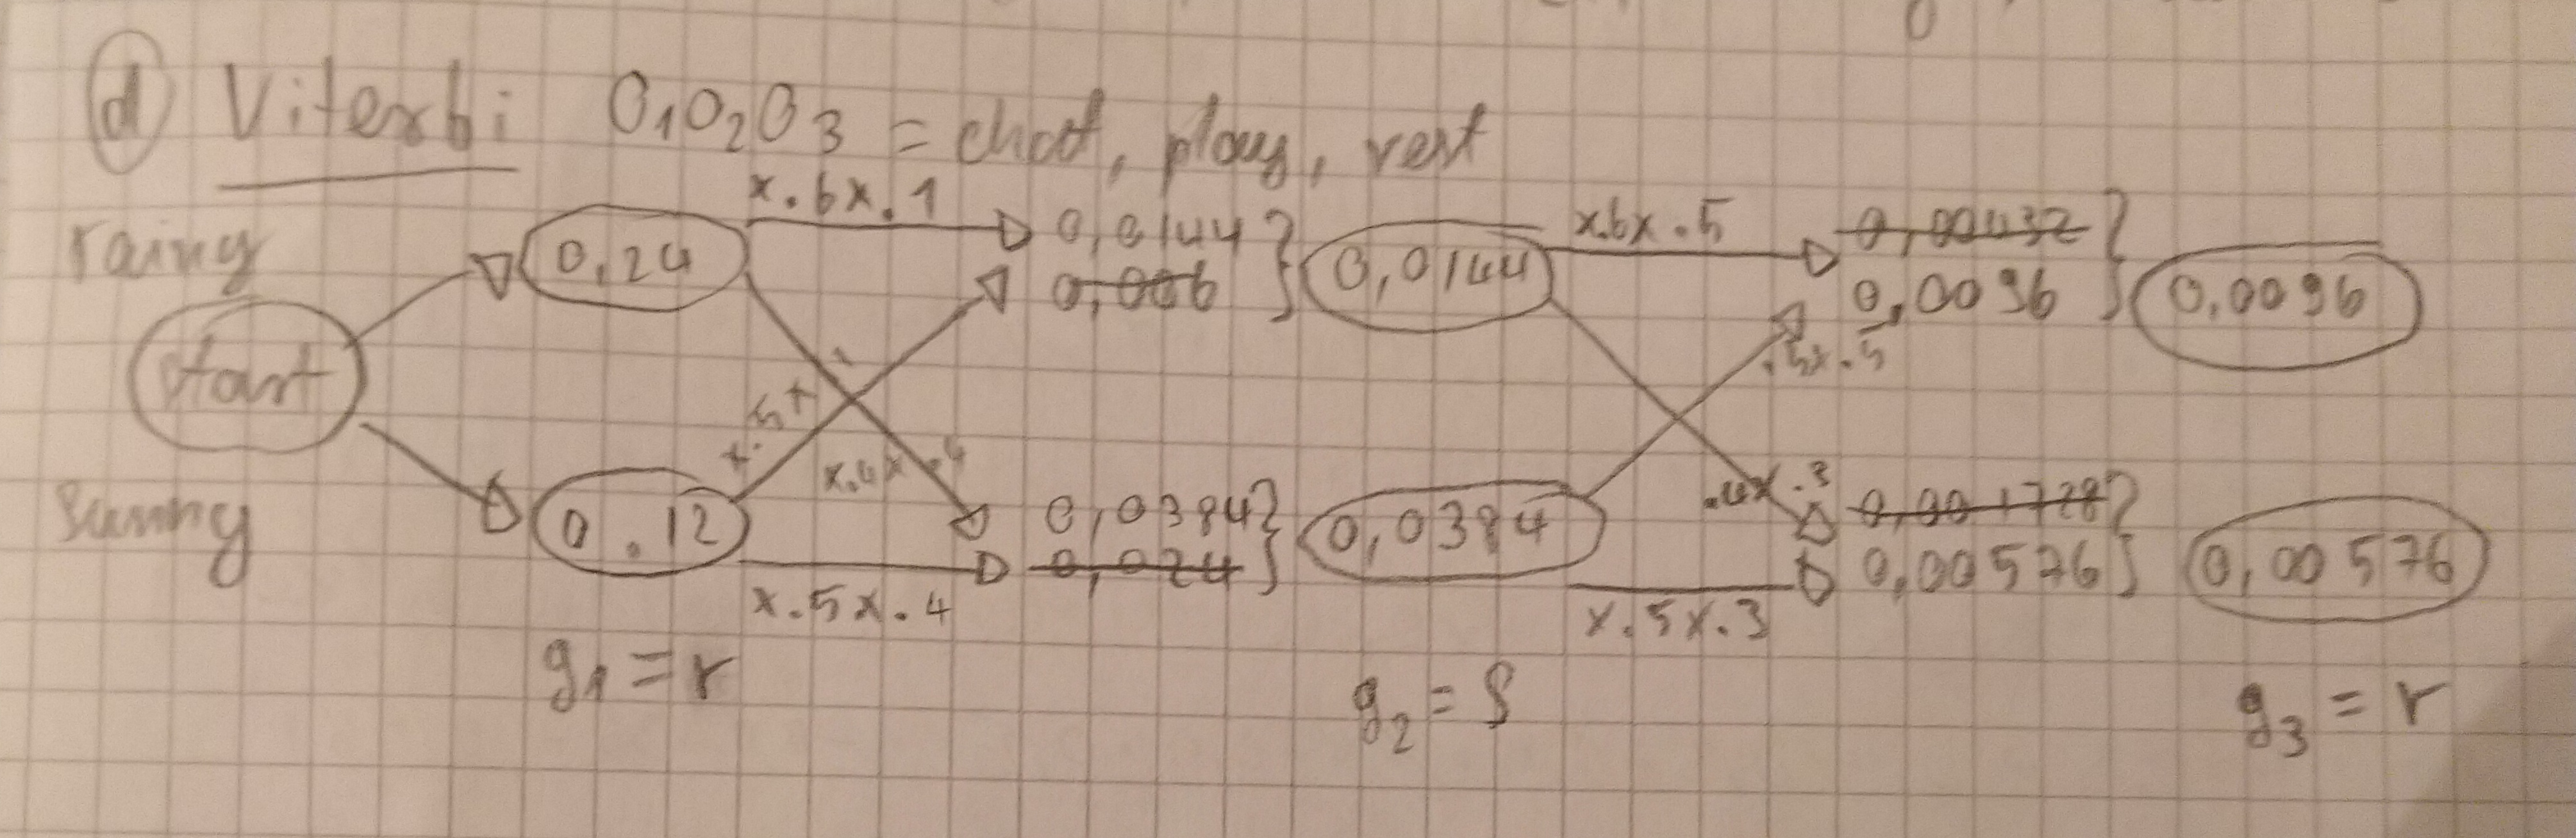
\includegraphics[width=.9\columnwidth]{viterbi}
\caption{Manual computation of the Viterbi Algorithm.}
\label{fig:viterbi-task1}
\end{figure}

Figure \ref{fig:viterbi-task1} shows the computation of the Viterbi Algorithm. The most probable set of states for the given observations is: \textit{rainy}, \textit{sunny}, \textit{rainy}.

\section{Task 2}
\subsection{Point a}
\begin{figure}[!ht]
\center
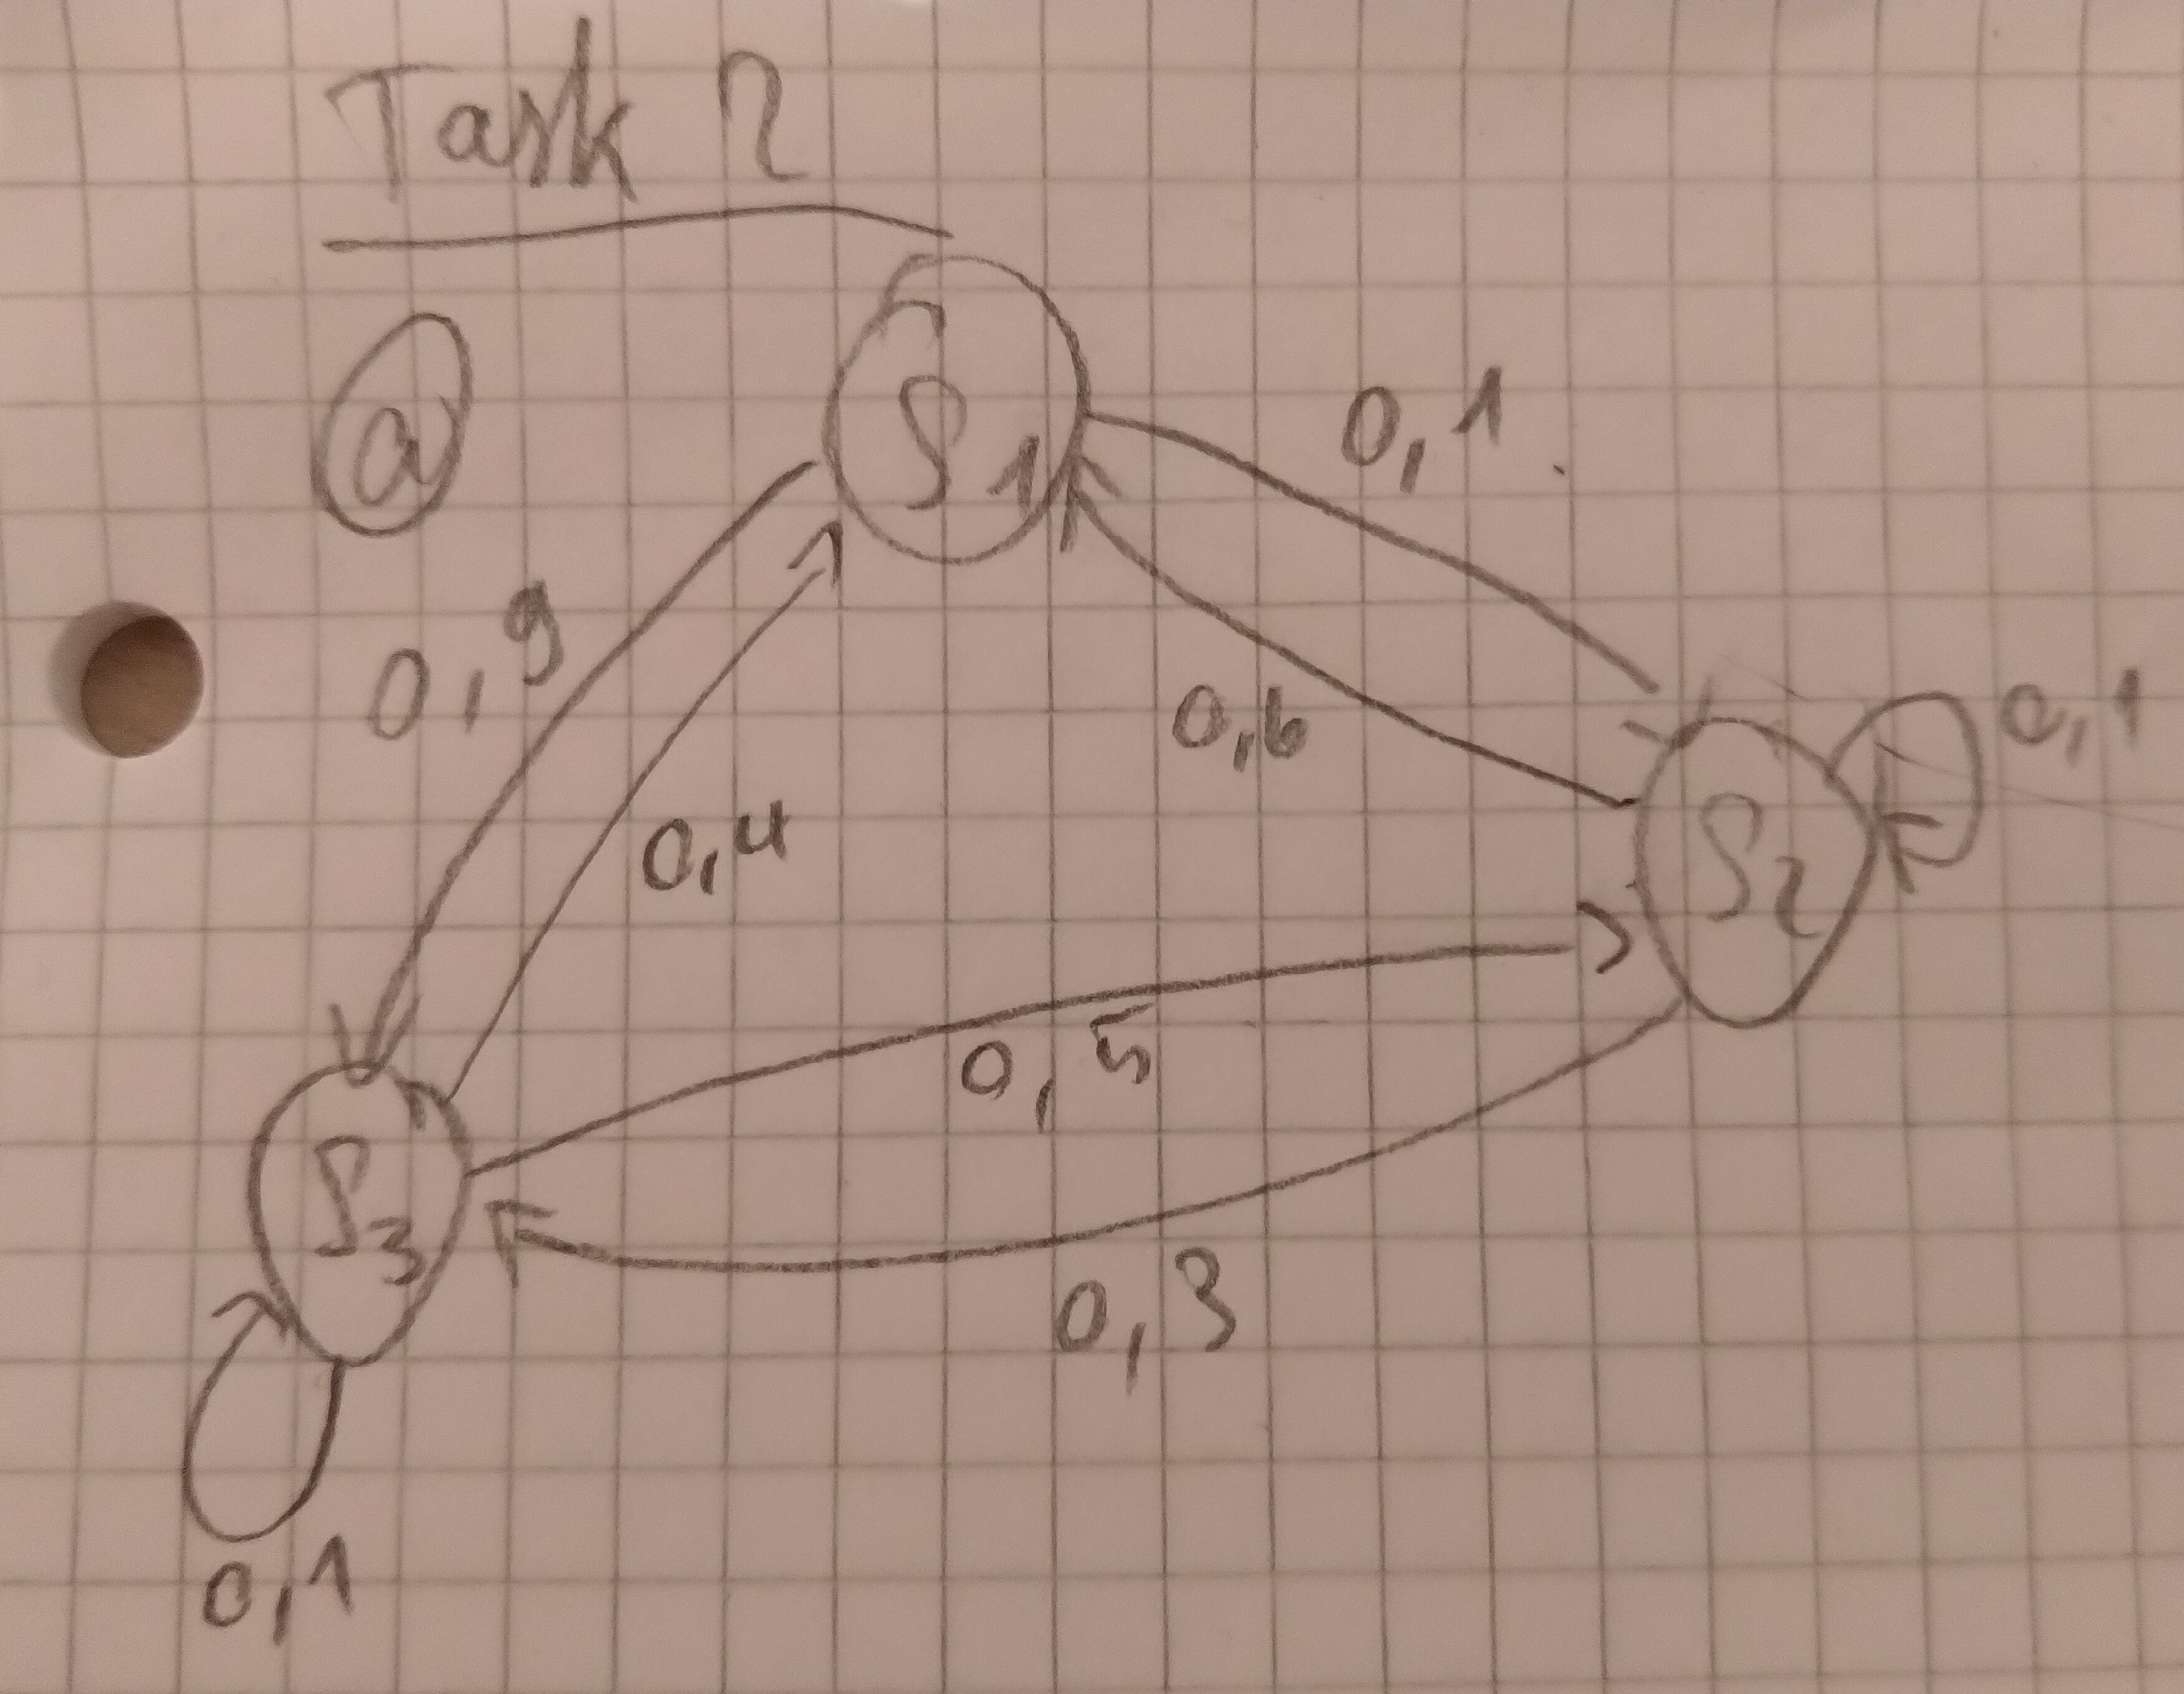
\includegraphics[width=.5\columnwidth]{chain_task2}
\caption{The schema of the Markov chain from the given probability matrix.}
\label{fig:chain-task2}
\end{figure}

Figure \ref{fig:chain-task2} shows a schema of the Markov chain.

\subsection{Point b}
The total number of state sequence is any permutation of the three states $S_1,S_2,S_3$ except the ones with two or more consecutive $S_1$ since $S_1$ cannot stay in $S_1$. \\
Total number of permutations $= 3^5 = 243$ sequences.
Number of permutations containing two or more consecutive $S_1 = 1 + 4 + 12 + 32 + 2 = 51 \leftrightarrow$ (5 $S_1$ + 4 $S_1$ preceded or followed by $S_2$ or $S_3$ + 3 $S1$ with any two other states + 2 $S_1$ with any 3 other states + two pairs of $S_1$ with one other state in between.) \\
Therefore the total number of possible sequences is $243 - 51 = 192$.

\subsection{Point c}
I used an iterative function to approximate the solution, the function stopped when the difference between the values at time $t$ and $t-1$ were less than \num{1e-9} .The Python code used to find the answer is part of the code submitted with this report. \\
The result obtained was: $P_s = \begin{pmatrix}
0.3235941 \\ 0.26470588 \\ 0.41176471
\end{pmatrix}$
\subsection{Point d}
Only did point 1 because I had problems with logarithm of probabilities.

\section{Task 3}
I did not have time.

\bibliography{biblio}
\bibliographystyle{unsrt}
\end{document}  

















